% GNUPLOT: LaTeX picture with Postscript
\begingroup
  \makeatletter
  \providecommand\color[2][]{%
    \GenericError{(gnuplot) \space\space\space\@spaces}{%
      Package color not loaded in conjunction with
      terminal option `colourtext'%
    }{See the gnuplot documentation for explanation.%
    }{Either use 'blacktext' in gnuplot or load the package
      color.sty in LaTeX.}%
    \renewcommand\color[2][]{}%
  }%
  \providecommand\includegraphics[2][]{%
    \GenericError{(gnuplot) \space\space\space\@spaces}{%
      Package graphicx or graphics not loaded%
    }{See the gnuplot documentation for explanation.%
    }{The gnuplot epslatex terminal needs graphicx.sty or graphics.sty.}%
    \renewcommand\includegraphics[2][]{}%
  }%
  \providecommand\rotatebox[2]{#2}%
  \@ifundefined{ifGPcolor}{%
    \newif\ifGPcolor
    \GPcolortrue
  }{}%
  \@ifundefined{ifGPblacktext}{%
    \newif\ifGPblacktext
    \GPblacktexttrue
  }{}%
  % define a \g@addto@macro without @ in the name:
  \let\gplgaddtomacro\g@addto@macro
  % define empty templates for all commands taking text:
  \gdef\gplbacktext{}%
  \gdef\gplfronttext{}%
  \makeatother
  \ifGPblacktext
    % no textcolor at all
    \def\colorrgb#1{}%
    \def\colorgray#1{}%
  \else
    % gray or color?
    \ifGPcolor
      \def\colorrgb#1{\color[rgb]{#1}}%
      \def\colorgray#1{\color[gray]{#1}}%
      \expandafter\def\csname LTw\endcsname{\color{white}}%
      \expandafter\def\csname LTb\endcsname{\color{black}}%
      \expandafter\def\csname LTa\endcsname{\color{black}}%
      \expandafter\def\csname LT0\endcsname{\color[rgb]{1,0,0}}%
      \expandafter\def\csname LT1\endcsname{\color[rgb]{0,1,0}}%
      \expandafter\def\csname LT2\endcsname{\color[rgb]{0,0,1}}%
      \expandafter\def\csname LT3\endcsname{\color[rgb]{1,0,1}}%
      \expandafter\def\csname LT4\endcsname{\color[rgb]{0,1,1}}%
      \expandafter\def\csname LT5\endcsname{\color[rgb]{1,1,0}}%
      \expandafter\def\csname LT6\endcsname{\color[rgb]{0,0,0}}%
      \expandafter\def\csname LT7\endcsname{\color[rgb]{1,0.3,0}}%
      \expandafter\def\csname LT8\endcsname{\color[rgb]{0.5,0.5,0.5}}%
    \else
      % gray
      \def\colorrgb#1{\color{black}}%
      \def\colorgray#1{\color[gray]{#1}}%
      \expandafter\def\csname LTw\endcsname{\color{white}}%
      \expandafter\def\csname LTb\endcsname{\color{black}}%
      \expandafter\def\csname LTa\endcsname{\color{black}}%
      \expandafter\def\csname LT0\endcsname{\color{black}}%
      \expandafter\def\csname LT1\endcsname{\color{black}}%
      \expandafter\def\csname LT2\endcsname{\color{black}}%
      \expandafter\def\csname LT3\endcsname{\color{black}}%
      \expandafter\def\csname LT4\endcsname{\color{black}}%
      \expandafter\def\csname LT5\endcsname{\color{black}}%
      \expandafter\def\csname LT6\endcsname{\color{black}}%
      \expandafter\def\csname LT7\endcsname{\color{black}}%
      \expandafter\def\csname LT8\endcsname{\color{black}}%
    \fi
  \fi
  \setlength{\unitlength}{0.0500bp}%
  \begin{picture}(7936.00,7936.00)%
    \gplgaddtomacro\gplbacktext{%
      \csname LTb\endcsname%
      \put(860,4319){\makebox(0,0)[r]{\strut{} 10}}%
      \put(860,4609){\makebox(0,0)[r]{\strut{} 20}}%
      \put(860,4900){\makebox(0,0)[r]{\strut{} 30}}%
      \put(860,5191){\makebox(0,0)[r]{\strut{} 40}}%
      \put(860,5482){\makebox(0,0)[r]{\strut{} 50}}%
      \put(860,5772){\makebox(0,0)[r]{\strut{} 60}}%
      \put(860,6063){\makebox(0,0)[r]{\strut{} 70}}%
      \put(860,6354){\makebox(0,0)[r]{\strut{} 80}}%
      \put(860,6644){\makebox(0,0)[r]{\strut{} 90}}%
      \put(860,6935){\makebox(0,0)[r]{\strut{} 100}}%
      \put(980,3828){\makebox(0,0){\strut{}}}%
      \put(1639,3828){\makebox(0,0){\strut{}}}%
      \put(2299,3828){\makebox(0,0){\strut{}}}%
      \put(2958,3828){\makebox(0,0){\strut{}}}%
      \put(3618,3828){\makebox(0,0){\strut{}}}%
      \put(4277,3828){\makebox(0,0){\strut{}}}%
      \put(4937,3828){\makebox(0,0){\strut{}}}%
      \put(5596,3828){\makebox(0,0){\strut{}}}%
      \put(6256,3828){\makebox(0,0){\strut{}}}%
      \put(6915,3828){\makebox(0,0){\strut{}}}%
      \put(7575,3828){\makebox(0,0){\strut{}}}%
      \put(160,5481){\rotatebox{-270}{\makebox(0,0){\strut{}max. Scanfehler [MHz]}}}%
    }%
    \gplgaddtomacro\gplfronttext{%
    }%
    \gplgaddtomacro\gplbacktext{%
      \csname LTb\endcsname%
      \put(863,1364){\makebox(0,0)[r]{\strut{}-6}}%
      \put(863,1727){\makebox(0,0)[r]{\strut{}-4}}%
      \put(863,2091){\makebox(0,0)[r]{\strut{}-2}}%
      \put(863,2454){\makebox(0,0)[r]{\strut{} 0}}%
      \put(863,2818){\makebox(0,0)[r]{\strut{} 2}}%
      \put(863,3181){\makebox(0,0)[r]{\strut{} 4}}%
      \put(863,3545){\makebox(0,0)[r]{\strut{} 6}}%
      \put(983,800){\makebox(0,0){\strut{}17:00}}%
      \put(1642,800){\makebox(0,0){\strut{}17:30}}%
      \put(2301,800){\makebox(0,0){\strut{}18:00}}%
      \put(2961,800){\makebox(0,0){\strut{}18:30}}%
      \put(3620,800){\makebox(0,0){\strut{}19:00}}%
      \put(4279,800){\makebox(0,0){\strut{}19:30}}%
      \put(4938,800){\makebox(0,0){\strut{}20:00}}%
      \put(5597,800){\makebox(0,0){\strut{}20:30}}%
      \put(6257,800){\makebox(0,0){\strut{}21:00}}%
      \put(6916,800){\makebox(0,0){\strut{}21:30}}%
      \put(7575,800){\makebox(0,0){\strut{}22:00}}%
      \put(403,2454){\rotatebox{-270}{\makebox(0,0){\strut{}FSR Fehler [MHz]}}}%
      \put(4279,500){\makebox(0,0){\strut{}Zeit}}%
    }%
    \gplgaddtomacro\gplfronttext{%
    }%
    \gplbacktext
    \put(0,0){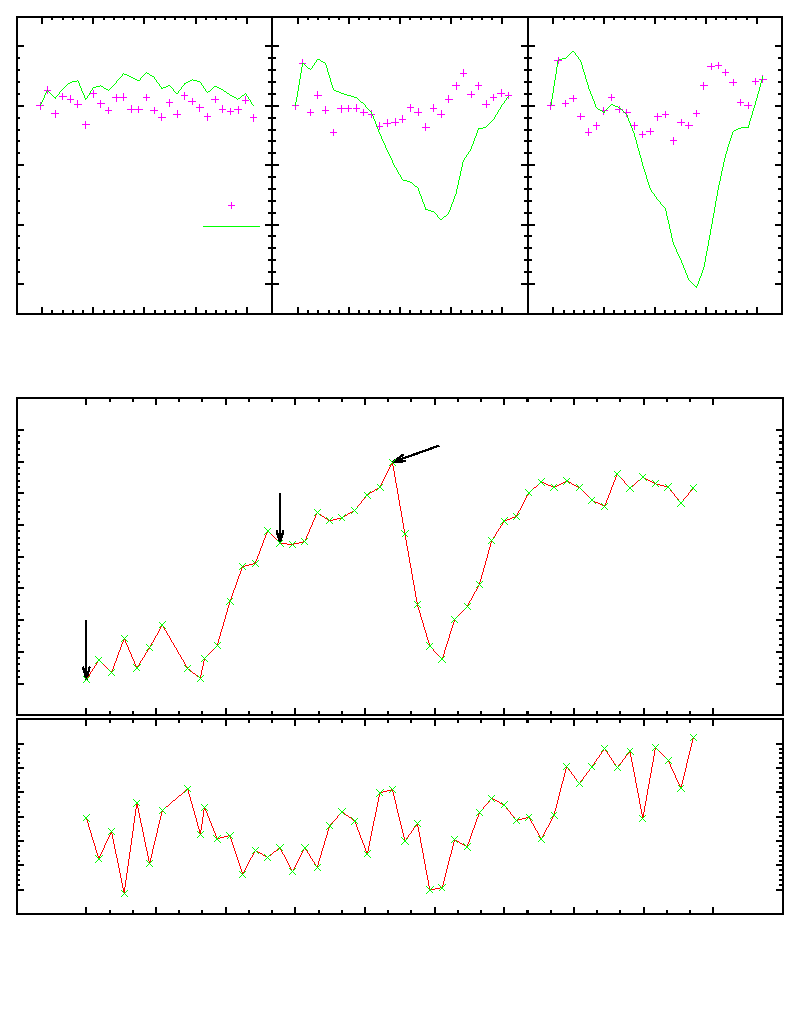
\includegraphics{linearitaet_verlauf}}%
    \gplfronttext
  \end{picture}%
\endgroup
